% ------------------------------------------------------------------------------
% TYPO3 CMS 8.5 - What's New - Chapter "In-Depth Changes" (German Version)
%
% @author	Michael Schams <schams.net>
% @license	Creative Commons BY-NC-SA 3.0
% @link		http://typo3.org/download/release-notes/whats-new/
% @language	English
% ------------------------------------------------------------------------------
% LTXE-CHAPTER-UID:		5ebcecbe-66abfa57-cf38bc00-aa637965
% LTXE-CHAPTER-NAME:	In-Depth Changes
% ------------------------------------------------------------------------------

\section{Änderungen im System}
\begin{frame}[fragile]
	\frametitle{Änderungen im System}

	\begin{center}\huge{Kapitel 3:}\end{center}
	\begin{center}\huge{\color{typo3darkgrey}\textbf{Änderungen im System}}\end{center}

\end{frame}

% ------------------------------------------------------------------------------
% LTXE-SLIDE-START
% LTXE-SLIDE-UID:		e5386eca-a1b322ac-9785356f-7566f543
% LTXE-SLIDE-ORIGIN:	bde270e6-ffef8544-ea472ed5-89ba8c3d English
% LTXE-SLIDE-TITLE:		#78581: FormEngine Data Providers
% ------------------------------------------------------------------------------

\begin{frame}[fragile]
	\frametitle{Änderungen im System}
	\framesubtitle{FormEngine Data Provider}

	\begin{itemize}
		\item Der FormEngine Data-Provider \texttt{TcaFlexFetch} wurde in \texttt{TcaFlexPrepare} integriert
		\item Dies betrifft ausschlielich Instanzen, in denen ein eigener Data-Provider mit Abhängigkeit zu \texttt{TcaFlexFetch} deklariert wurde
	\end{itemize}

\end{frame}

% ------------------------------------------------------------------------------
% LTXE-SLIDE-START
% LTXE-SLIDE-UID:		5ba0aae0-2f93c4a2-34619663-2581fc4d
% LTXE-SLIDE-ORIGIN:	f0fb603c-54e9f255-03140395-b6b18103 English
% LTXE-SLIDE-TITLE:		#78384: Frontend ignores TCA in ext_tables.php
% ------------------------------------------------------------------------------
\begin{frame}[fragile]
	\frametitle{Änderungen im System}
	\framesubtitle{TCA in \texttt{ext\_tables.php}}

	\begin{itemize}
		\item Frontend-Requests laden nun nicht mehr \texttt{ext\_tables.php}
		\item Dies betrifft Extensions, die das TCA über \texttt{ext\_tables.php} konfigurieren\newline
			\small(was ohnehin nicht mehr gemacht werden sollte)\normalsize
		\item Das Install Tool stellt einen Test "TCA ext\_tables check" zur Verfügung, um solche Extensions herauszufinden
	\end{itemize}

	\begin{figure}
		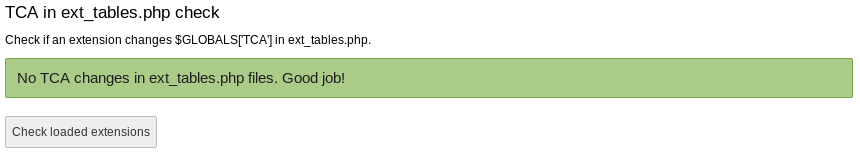
\includegraphics[width=0.95\linewidth]{InDepthChanges/78384-install-tool-tca-in-exttables-check.png}
	\end{figure}

\end{frame}
% ------------------------------------------------------------------------------
% LTXE-SLIDE-START
% LTXE-SLIDE-UID:		d92603a7-5f46543c-545d08a4-e3282867
% LTXE-SLIDE-ORIGIN:	bdcd2449-b679717b-9f23eb32-018953b4 English
% LTXE-SLIDE-TITLE:		#78191: Remove support for transForeignTable/transOrigPointerTable in TCA
% ------------------------------------------------------------------------------
\begin{frame}[fragile]
	\frametitle{Änderungen im System}
	\framesubtitle{TCA in \texttt{ext\_tables.php}}

	\begin{itemize}
		\item Das TCA erlaubte die Konfiguration von lokalisierten und übersetzten Datensätzen.

			\begin{itemize}
				\item \texttt{\$TCA[<table\_name>]['ctrl']['transForeignTable']}\newline
					(zeigt normalerweise auf: \texttt{pages\_language\_overlay})
				\item \texttt{\$TCA[<table\_name>]['ctrl']['transOrigPointerTable']}\newline
					(zeigt normalerweise auf: \texttt{pages})
			\end{itemize}

		\item Da in Zukunft nur noch eine \texttt{pages} Tabelle existieren soll und man Spezialbehandlungen
			verhindern will, wurde das obige Handling enfernt.

	\end{itemize}

\end{frame}

% ------------------------------------------------------------------------------
% LTXE-SLIDE-START
% LTXE-SLIDE-UID:		0bf5f47c-39abcfcf-e7a27e10-34250fcb
% LTXE-SLIDE-ORIGIN:	ede02440-cafd3417-eb416f09-8e024ef2 English
% LTXE-SLIDE-TITLE:		#78383: Tables removed from defaultCategorizedTables
% ------------------------------------------------------------------------------
\begin{frame}[fragile]
	\frametitle{Änderungen im System}
	\framesubtitle{Tabellen von \texttt{defaultCategorizedTables} entfernt}

	\begin{itemize}
		\item Die folgenden Tabellen wurden aus \texttt{defaultCategorizedTables} entfernt:

			\begin{itemize}
				\item \texttt{pages}
				\item \texttt{tt\_content}
				\item \texttt{sys\_file\_metadata}
			\end{itemize}

		\item Für diese Tabellen wird die Core API\newline
			\texttt{ExtensionManagementUtility::makeCategorizable()}\newline
			ausgeführt, um die Position des "categories" Feld zu definieren.

	\end{itemize}

\end{frame}


% ------------------------------------------------------------------------------
% LTXE-SLIDE-START
% LTXE-SLIDE-UID:		71571789-30a5acc4-542c97f2-e979d091
% LTXE-SLIDE-ORIGIN:	dd31e5d5-ca09ae5e-eb87d926-0ffe8f0a English
% LTXE-SLIDE-TITLE:		Low-level parameters changes (1)
% ------------------------------------------------------------------------------
\begin{frame}[fragile]
	\frametitle{Änderungen im System}
	\framesubtitle{Low-level Parameter Changes (1)}

	% changes: #78417, #78439, #78520, #78552, #78577, #78623, #78627 and #78895

	\begin{itemize}
		\item Die nachfolgenden Low-Level Befehle verwenden nun die Symfony Console
		\item Die neuen Befehle verhalten sich wie die alten - allerdings mit zusätzlichen Parametern

			\begin{itemize}
				\item \texttt{DeletedRecordsCommand}
				\item \texttt{CleanFlexFormsRecordsCommand}
				\item \texttt{OrphanRecordsCommand}
				\item \texttt{LostFilesCommand}
				\item \texttt{MissingFilesCommand}
				\item \texttt{MissingRelationsCommand}
				\item \texttt{DoubleFilesCommand}
				\item \texttt{RteImagesCommand}
			\end{itemize}

	\end{itemize}

\end{frame}



% ------------------------------------------------------------------------------
% LTXE-SLIDE-START
% LTXE-SLIDE-UID:		4096bcad-a2cb831e-0ac0ad6b-916240c1
% LTXE-SLIDE-ORIGIN:	3a9d25bb-d948368d-e2a92666-6170eaad English
% LTXE-SLIDE-TITLE:		Low-level parameters changes (2)
% ------------------------------------------------------------------------------
\begin{frame}[fragile]
	\frametitle{Änderungen im System}
	\framesubtitle{Low-level Parameter Changes (2)}

	% changes: #78417, #78439, #78520, #78552, #78577, #78623, #78627 and #78895

	\begin{itemize}
		\item Es wurden entsprechende PHP-Klassen entfernt\newline
			\smaller(z.B. \texttt{TYPO3\textbackslash
				CMS\textbackslash
				Lowlevel\textbackslash
				DeletedRecordsCommand})
			\normalsize

		\item Die Ausführung via \texttt{cli\_dispatch} funktioniert nicht mehr\newline
			\smaller(z.B. \texttt{typo3/cli\_dispatch lowlevel cleaner deleted})\normalsize
		\item Der Aufruf der PHP-Klasse sorgt nun für einen PHP-Fehler

		\item Befehle werden nun per CLI wie folgt ausgeführt:\newline
			\smaller\texttt{/typo3/sysext/core/bin/typo3 cleanup:<command>}\normalsize\newline
			zum Beispiel:\newline
			\smaller\texttt{/typo3/sysext/core/bin/typo3 cleanup:deletedrecords}\normalsize

	\end{itemize}

\end{frame}




% ------------------------------------------------------------------------------
% LTXE-SLIDE-START
% LTXE-SLIDE-UID:		de4a6eb0-c8362945-b0d4f178-7f299fc8
% LTXE-SLIDE-ORIGIN:	ec6817fd-c3364ffb-c74e9523-a18a3095 English
% LTXE-SLIDE-TITLE:		Re-factor FlexForm Data Structure Handling
% ------------------------------------------------------------------------------
\begin{frame}[fragile]
	\frametitle{Änderungen im System}
	\framesubtitle{Refactoring des FlexForm Data Structure Handlings}

	% https://forge.typo3.org/issues/78581
	% https://forge.typo3.org/issues/78616
	% https://forge.typo3.org/issues/78852
	% https://forge.typo3.org/issues/69715

	\begin{itemize}
		\item Nachdem \texttt{BackendUtility::getFlexFormDS()} als veraltet gilt, wird auch der Hook
			\texttt{getFlexFormDSClass} nicht mehr aufgerufen

	\end{itemize}

\end{frame}





% ------------------------------------------------------------------------------
% LTXE-SLIDE-START
% LTXE-SLIDE-UID:		cebc3663-6daaaf89-a92f3a76-047a4607
% LTXE-SLIDE-ORIGIN:	b400c3b8-3e402480-cd7d6ff3-96cd93aa English
% LTXE-SLIDE-TITLE:		#76085: Add fluid debug information to admin panel
% ------------------------------------------------------------------------------
\begin{frame}[fragile]
	\frametitle{Änderungen im System}
	\framesubtitle{Admin Panel}

	\begin{itemize}
		\item Das Admin Panel hat eine neue Einstellungen, um Fluid besser debuggen zu können:\newline
			\textbf{Preview -> Show fluid debug output}
		\item Wenn dies aktiviert ist, werden folgende Informationen im Frontend angezeigt:

			\begin{itemize}
				\item Pfad zur Partial Template Datei
				\item Name der Section
			\end{itemize}

		\item Damit kann der Integrator leichter die richtigen Templates und Sections identifizieren
	\end{itemize}

\end{frame}






% ------------------------------------------------------------------------------
% LTXE-SLIDE-START
% LTXE-SLIDE-UID:		5fba7ce4-b00101c1-a8292115-9743836b
% LTXE-SLIDE-ORIGIN:	60a2d39f-f04b8bf1-dc758912-607ed07e English
% LTXE-SLIDE-TITLE:		#52286: System Status Updates Report via email
% ------------------------------------------------------------------------------
\begin{frame}[fragile]
	\frametitle{Änderungen im System}
	\framesubtitle{System Status Updates (Reports)}

	\begin{itemize}
		\item Die Resultate des Tests "System Status Updates (reports)" können nun per Mail versendet werden
		\item Es wurde eine Checkbox hinzugefügt:

			\begin{itemize}
				\item Sende Email bei Warnungen und Fehlern
				\item Immer eine Email senden
			\end{itemize}

		\item Die erste Option ist der Default-Wert

	\end{itemize}

\end{frame}







% ------------------------------------------------------------------------------
% LTXE-SLIDE-START
% LTXE-SLIDE-UID:		5a2fec12-43481107-bbd17933-e6ae34dd
% LTXE-SLIDE-ORIGIN:	e4e2ead3-c07beb21-e8100580-d0e7c756 English
% LTXE-SLIDE-TITLE:		#58637: Purge language packs in language module
% ------------------------------------------------------------------------------
\begin{frame}[fragile]
	\frametitle{Änderungen im System}
	\framesubtitle{Sprachpakete}

	\begin{itemize}
		\item Die Deaktivierung von Sprachpaketen Modul "Languages" hinterlässt die Sprachdaten im Verzeichnis
			\texttt{typo3conf/l10n/<locale>/}
		\item Es wurde ein "Entfernen"-Button zugefügt, mit dem die Daten entfernt werden können
	\end{itemize}

\end{frame}








% ------------------------------------------------------------------------------
% LTXE-SLIDE-START
% LTXE-SLIDE-UID:		60051e5e-062ae5e0-da8664c0-e8e30814
% LTXE-SLIDE-ORIGIN:	08961fb3-00cbc9f4-964f8d01-6e59e782 English
% LTXE-SLIDE-TITLE:		#67909: Hook added to localize() function
% ------------------------------------------------------------------------------
\begin{frame}[fragile]
	\frametitle{Änderungen im System}
	\framesubtitle{Hook im DataHandler \texttt{localize()}}

	% decrease font size for code listing
	\lstset{basicstyle=\tiny\ttfamily}

	\begin{itemize}
		\item Es wurde ein neuer Hook zur \texttt{localize()} Funktion hinzugefügt
		\item Dieser erlaubt beispielsweise die Verwendung eines externen Übersetzungsservice oder eines Transformationsservice
	\end{itemize}

	\begin{itemize}
		\item Hook:\newline
			\smaller
				\texttt{\$GLOBALS['TYPO3\_CONF\_VARS']['SC\_OPTIONS']\newline
				\tabto{0.4cm}['t3lib/class.t3lib\_tcemain.php']['processTranslateToClass']}
			\normalsize

		\item Beispiel:

			\begin{lstlisting}
				class YourHookClass
				{
				  public function processTranslateTo_copyAction(&$content, $lang, $dataHandler)
				  {
				    // Veraendern den Inhalts (uebersetzen, transkribieren u.s.w.)
				  }
				}
			\end{lstlisting}
	\end{itemize}

\end{frame}









% ------------------------------------------------------------------------------
% LTXE-SLIDE-START
% LTXE-SLIDE-UID:		70f0b744-f625847f-ae7c1895-11c7811a
% LTXE-SLIDE-ORIGIN:	8b1a9661-d6fab90f-9c856224-ee663aa2 English
% LTXE-SLIDE-TITLE:		#77757: Re-check if an UpdateWizard should run
% ------------------------------------------------------------------------------
\begin{frame}[fragile]
	\frametitle{Änderungen im System}
	\framesubtitle{Update Wizard}

	\begin{columns}[T]
		\begin{column}{.5\textwidth}
			Der Update Wizard im Install Tool listet nun alle Tasks auf, die als \textit{completed} markiert wurden.
			\newline\newline
			Checkboxen und ein Button "Recheck chosen wizards" erlauben nun die Updates erneut durchzuführen.
			Der Wizard testet ob der Task erneut ausgeführt werden sollte.
		\end{column}
		\begin{column}{.5\textwidth}
			\begin{figure}\vspace*{-0.5cm}
				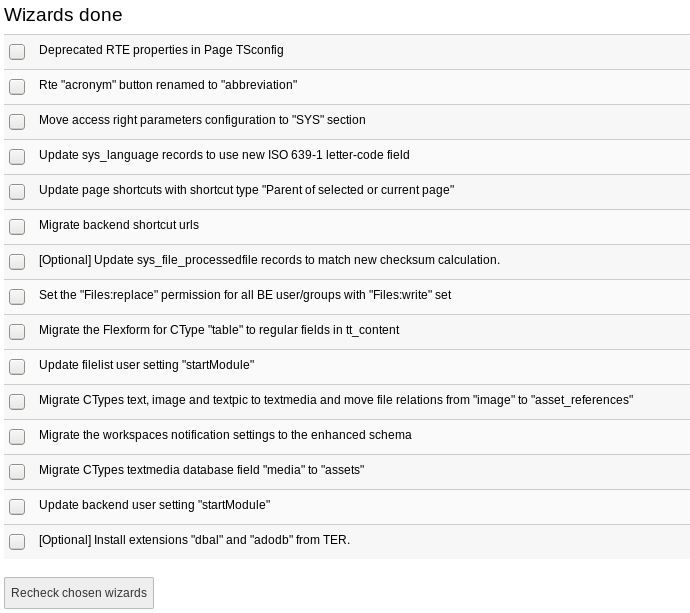
\includegraphics[width=0.8\linewidth]{InDepthChanges/77757-upgrade-wizard.png}
			\end{figure}
		\end{column}
	\end{columns}

\end{frame}









% ------------------------------------------------------------------------------
% LTXE-SLIDE-START
% LTXE-SLIDE-UID:		c8652313-b5819309-b03ecfb5-ba837a2a
% LTXE-SLIDE-ORIGIN:	94640f3d-0f632507-a2166719-5adc755e English
% LTXE-SLIDE-TITLE:		#78523: Suggest wizard provides option to define ordering of results
% ------------------------------------------------------------------------------
\begin{frame}[fragile]
	\frametitle{Änderungen im System}
	\framesubtitle{Suggest Wizard}

	% decrease font size for code listing
	\lstset{basicstyle=\tiny\ttfamily}

	\begin{itemize}
		\item Innerhalb der FormEngine ("TCEforms") kann man nun die Reihenfolge der Resultate konfigurieren
		\item Die neue Option folgt nun der Standard-SQL "order-by" Definition:\newline
			\small\texttt{'orderBy' => 'field ASC/DESC'}\normalsize
		\item Beispielhafte TCA-Konfiguration:

			\begin{lstlisting}
				'config' => [
				  ...
				  'wizards' => [
				    'suggest' => [
				      'type' => 'suggest',
				      'default' => [
				        'searchWholePhrase' => true,
				        'addWhere' => ' AND tx_news_domain_model_news.uid != ###THIS_UID###',
				        'orderBy => 'datetime DESC',
				      ]
				    ],
				  ],
				]
			\end{lstlisting}

	\end{itemize}

\end{frame}


% ------------------------------------------------------------------------------
% LTXE-SLIDE-START
% LTXE-SLIDE-UID:		13b52b1a-63a20add-e35701ae-bc2d2639
% LTXE-SLIDE-ORIGIN:	0907e5d3-a12751cb-23f49488-7a05a208 English
% LTXE-SLIDE-TITLE:		Miscellaneous
% ------------------------------------------------------------------------------
\begin{frame}[fragile]
	\frametitle{Änderungen im System}
	\framesubtitle{Misc}

	% #78103: Add missing information status for addSystemMessage
	% #78575: Get enumeration constants
	% #75232: Spread TypeConverter priorities

	\begin{itemize}
		\item Die System-Informationen durch \texttt{addSystemInformation()} haben nun den Default-Wert
			\texttt{InformationStatus::STATUS\_NOTICE}
		\item Aufzählungs-Konstanten können nun wie folgt verwendet werden:

			\begin{itemize}
				\item \texttt{EnumerationClass::getName(\$value);}
				\item \texttt{EnumerationClass::getHumanReadableName(\$value);}
			\end{itemize}

		\item Die Prioritäten der Core TypeConverter wurden geändert von\newline
			\texttt{1}, \texttt{2}, \texttt{3},... in \texttt{10}, \texttt{20}, \texttt{30},...
			Bei der Registrierung von eigenen TypeConverter muss man sicherstellen, dass diese die korrekte Priorität verwenden.

		\item \href{https://en.wikipedia.org/wiki/ISO_8601}{ISO-8601} wird verwendet um "date" sowie "datetime" Werte zwischen Server und Client auszutauschen. Es muss überprüft werden, ob eigene FormEngine Render Types zu \texttt{eval=date/datetime} aktualisiert werden müssen.

	\end{itemize}

\end{frame}

% ------------------------------------------------------------------------------
